\begin{comment}
\documentclass{article}
\usepackage[utf8]{inputenc}
\usepackage{graphicx}
\usepackage{hyperref}
\usepackage{float}


\DeclareGraphicsExtensions{.jpg}
\graphicspath{{./Images/}}
\end{comment}

	
%\newcommand{\HRule}{\rule{\linewidth}{0.5mm}}
\begin{titlepage}
\begin{center}

\includegraphics[width = 0.3\textwidth]{US_newLogo.png}~\\[1cm]
\textsc{\LARGE Unsolvable Solutions}\\
Client: Francois Mouton at the CSIR DSSR\\[1.5cm]
\textsc{\Large  Architectural Requirements}\\[0.5cm]

 \HRule\\[0.4cm]
{ \huge \bfseries  Eavesdrop \\[0.4cm] }

 \HRule\\ 



Github link:  \url{https://github.com/Unsolvable-Solutions/Project-EPIC} \\[1.2cm]

\noindent
\begin{minipage}[t]{0.4\textwidth}

	\begin{flushleft} \large
	\emph{Members:}\\
		Edwin Fullard  \\
		Jaco Bezuidenhoudt \\
		Jandre Coetzee\\
		Maret Stoffberg\\
		Ryno Pierce\\
	\end{flushleft}
\end{minipage}%
\begin{minipage}[t]{0.4\textwidth}
\begin{flushright} \large
	\emph{Student Number:} \\
		12048675 \\
		11013878 \\
		 10693077 \\
		 11071762 \\
		 12003922\\
	\end{flushright}
\end{minipage}

\vfill


% Bottom of the page




\end{center}
\end{titlepage}


	
	% Table of content
	\newpage
	\tableofcontents
	\newpage
	\section{Introduction}
	\subsection{Project Background}

The Android Operating System officially took over the smart phone market in 2010 and it is suspected that about 700 000 Android devices are used in South Africa. It is mostly the corporate or more upper class communities that have access to these smart phone devices. It is also these individuals who sit in the big corporate meetings where extremely sensitive data can be discussed. For this reason, if these individuals should have eavesdropping malicious software(malware) on their smart phone, it could cause sensitive data to be easily leaked out.


		\subsection{Project Vision}
The aim of the malware is to eavesdrop on a person via their own smart phone. This is done by live streaming the conversation from the infected smartphone to a remote server which plays back the stream and saves a local copy of the recording on the server.
		\subsection{Project Scope}
The malware consist of a webserver that connects with the mobile device via a web socket. A request is send from the server to the application on the mobile device to start recording. The mobile device will start to stream live to the server which in turn plays back the stream and creates a local recording.

	%  The functional requirements
\newpage


	\section{Functional Requirements}
		\begin{figure}[H]
 			 \centering
			  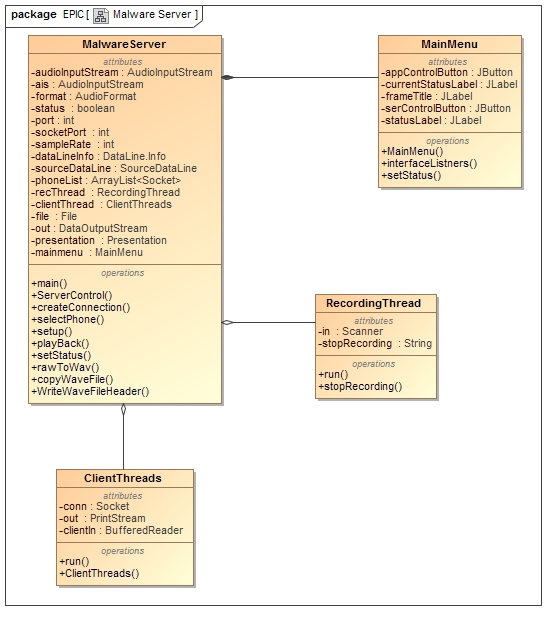
\includegraphics[width=12cm]{MalwareClass}
		 	 \caption{A Class Diagram of the Malware}
		\end{figure}
		
\begin{comment}
Template vir elke funksie
        \paragraph{}
			\begin{description}
			    \item{\textbf{Priority}:} %watter prioriteit dit het: Critical, Important of Nic-to-have
			    \item{\textbf{Service Contract}:}% Wat dit doen
			    \item{\textbf{Pre-conditions}:}%wat moet waar wees voor die funksie sy ding kan doen
    			    \begin{itemize}
    			        \item %precondition 1
    			        \item %precondition 2
    			    \end{itemize}
			    \item{\textbf{Post-conditions}:} % wat moet waar wees na die funksie sy ding gedoen het
    			    \begin{itemize}
    			    \item %post condition 1
    			    \item %post condition2
    			    \end{itemize}
			\end{description}
\end{comment}




\subsection{Malware Server}

    \subsubsection{Scope}
	With the server the user will be able to target a specific android device to start recording and streaming the data back to the server.
		\begin{figure}[H]
 			 \centering
			  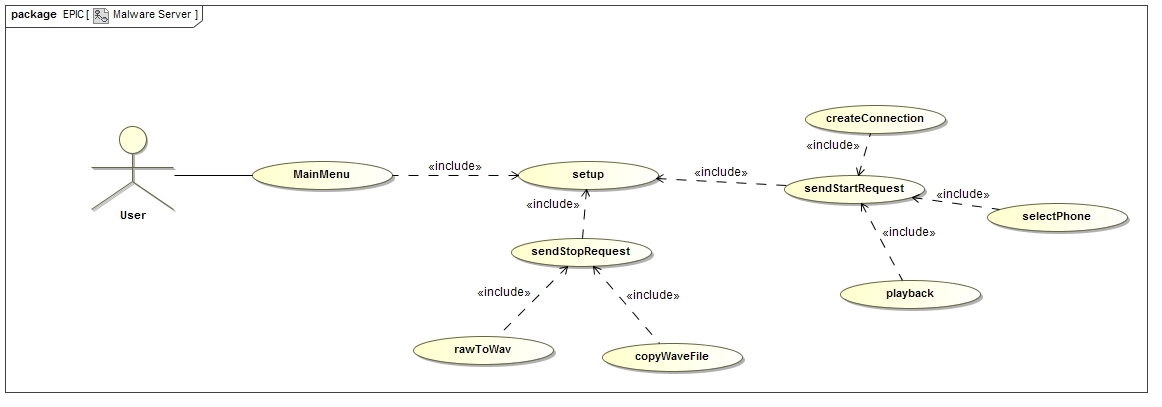
\includegraphics[width=12cm]{MalwareServerUseCase}
		 	 \caption{A Use Case Diagram of the Malware Server}
		\end{figure}
	
	
	\subsubsection{Functionality}
   
        \paragraph{sendStartRequest}
			\begin{description}
			    \item{\textbf{Priority}:} Critical%watter prioriteit dit het: Critical, Important of Nic-to-have
			    \item{\textbf{Service Contract}:}
			    This service will send a request to a specific mobile device that has the malware application installed to start a live stream.
			    \item{\textbf{Pre-conditions}:}%wat moet waar wees voor die funksie sy ding kan doen
    			    \begin{itemize}
    			        \item The malware application has created a connection with the server.
    			        \item The setup modules has been initialised.
    			    \end{itemize}
			    \item{\textbf{Post-conditions}:} % wat moet waar wees na die funksie sy ding gedoen het
    			    \begin{itemize}
    			    \item Receive the live stream.
    			    \end{itemize}
			\end{description}

    
         \paragraph{sendStopRequest}
			\begin{description}
			    \item{\textbf{Priority}:} Critical%watter prioriteit dit het: Critical, Important of Nic-to-have
			    \item{\textbf{Service Contract}:} This service sends a request to the malware application on a specified device to stop the live streaming.% Wat dit doen
			    \item{\textbf{Pre-conditions}:}%wat moet waar wees voor die funksie sy ding kan doen
    			    \begin{itemize}
    			        \item The server must be busy recording a live steam.
    			        \item The setup modules has been initialised.
    			    \end{itemize}
			    \item{\textbf{Post-conditions}:} % wat moet waar wees na die funksie sy ding gedoen het
    			    \begin{itemize}
    			    \item A stop request was sent to the malware application on the remote mobile device.
    			    \item A local recording of the live stream was stored on the server.
    			    \end{itemize}
			\end{description}
		
		
		\paragraph{playback}
			\begin{description}
			    \item{\textbf{Priority}:} Critical%watter prioriteit dit het: Critical, Important of Nic-to-have
			    \item{\textbf{Service Contract}:} The recorded stream is played back to the user over the speakers.% Wat dit doen
			    \item{\textbf{Pre-conditions}:}%wat moet waar wees voor die funksie sy ding kan doen
    			    \begin{itemize}
    			        \item The server must be busy recording a live steam.
    			        \item The setup modules has been initialised.
    			    \end{itemize}
			    \item{\textbf{Post-conditions}:} % wat moet waar wees na die funksie sy ding gedoen het
    			    \begin{itemize}
    			    \item A stop request was sent to the malware application on a specified device.
    			    \item The RecordingThread thread was closed.
    			    \end{itemize}
			\end{description}
	
	
        \paragraph{setup}
			\begin{description}
			    \item{\textbf{Priority}:}Critical %watter prioriteit dit het: Critical, Important of Nic-to-have
			    \item{\textbf{Service Contract}:} Initialise the audio recording modules. Creates a recording thread to handle the live stream and to create a local copy of the stream.% Wat dit doen
			    \item{\textbf{Pre-conditions}:}%wat moet waar wees voor die funksie sy ding kan doen
    			    \begin{itemize}
    			        \item The malware application has created a connection with the server.
    			    \end{itemize}
			    \item{\textbf{Post-conditions}:} % wat moet waar wees na die funksie sy ding gedoen het
    			    \begin{itemize}
    			    \item A RecordingThread thread was created.
    			    \item Playback has been initialised.
    			    \end{itemize}
			\end{description}
			
			
        \paragraph{selectPhone}
			\begin{description}
			    \item{\textbf{Priority}:} Critical%watter prioriteit dit het: Critical, Important of Nic-to-have
			    \item{\textbf{Service Contract}:} Creates a list for selection of a device to stream and record from.% Wat dit doen
			    \item{\textbf{Pre-conditions}:}%wat moet waar wees voor die funksie sy ding kan doen
    			    \begin{itemize}
    			        \item The malware application has created a connection with the server.
    			        \item A ClientThreads thread exists which handles the connections
    			    \end{itemize}
			    \item{\textbf{Post-conditions}:} % wat moet waar wees na die funksie sy ding gedoen het
    			    \begin{itemize}
    			    \item The setup modules has been initialised.
    			    \item A RecordingThread thread was created.
    			    \end{itemize}
			\end{description}
	
	
        \paragraph{createConnection}
			\begin{description}
			    \item{\textbf{Priority}:} Critical%watter prioriteit dit het: Critical, Important of Nic-to-have
			    \item{\textbf{Service Contract}:} Provides the means to create a list of devices to connect to and to create the connection to a mobile device running the malware application.% Wat dit doen
			    \item{\textbf{Pre-conditions}:}%wat moet waar wees voor die funksie sy ding kan doen
    			    \begin{itemize}
    			        \item Ports 4545 and 8080 must be allowed in the firewall
    			        \item The server is not currently receiving a live stream.
    			    \end{itemize}
			    \item{\textbf{Post-conditions}:} % wat moet waar wees na die funksie sy ding gedoen het
    			    \begin{itemize}
    			    \item A ClientThreads thread was created. 
    			    \item The connection to a mobile device running the malware application was successful.
    			    \end{itemize}
			\end{description}
	
	
        \paragraph{rawToWav}
			\begin{description}
			    \item{\textbf{Priority}:} Important%watter prioriteit dit het: Critical, Important of Nic-to-have
			    \item{\textbf{Service Contract}:} Converts the RAW audio file to a WAVE file. 	% Wat dit doen
			    \item{\textbf{Pre-conditions}:}%wat moet waar wees voor die funksie sy ding kan doen
    			    \begin{itemize}
    			        \item A stop request was sent to the malware application on the remote mobile device.
    			        \item The RecordingThread thread was closed.
    			    \end{itemize}
			    \item{\textbf{Post-conditions}:} % wat moet waar wees na die funksie sy ding gedoen het
    			    \begin{itemize}
    			    \item The RAW audio file was removed
    			    \end{itemize}
			\end{description} 
	
	
        \paragraph{copyWaveFile}
			\begin{description}
			    \item{\textbf{Priority}:} Important%watter prioriteit dit het: Critical, Important of Nic-to-have
			    \item{\textbf{Service Contract}:}Takes the WAVE file and adds the required header to the file to enable correct playback.% Wat dit doen
			    \item{\textbf{Pre-conditions}:}%wat moet waar wees voor die funksie sy ding kan doen
    			    \begin{itemize}
    			        \item The RAW audio file was converted to a WAVE file
    			        \item The RAW audio file was removed
    			    \end{itemize}
			    \item{\textbf{Post-conditions}:} % wat moet waar wees na die funksie sy ding gedoen het
    			    \begin{itemize}
    			    \item The required header values was added to the wave file. 
    			    \end{itemize}
			\end{description}
	
        \paragraph{MainMenu}
			\begin{description}
			    \item{\textbf{Priority}:} Nice to have%watter prioriteit dit het: Critical, Important of Nic-to-have
			    \item{\textbf{Service Contract}:} Creates a user friendly interface for using the server.% Wat dit doen
			    \item{\textbf{Pre-conditions}:}%wat moet waar wees voor die funksie sy ding kan doen
    			    \begin{itemize}
    			        \item No previous interface exists.
    			    \end{itemize}
			    \item{\textbf{Post-conditions}:} % wat moet waar wees na die funksie sy ding gedoen het
    			    \begin{itemize}
    			    \item Interface listeners are active
    			    \item Main menu is visible.
    			    \end{itemize}
			\end{description}
	   	
				
        
\begin{comment}
Template vir elke funksie
    \paragraph{Funksie naam}
			\begin{description}
			    \item{\textbf{Priority}:} %watter prioriteit dit het: Critical, Important of Nic-to-have
			    \item{\textbf{Service Contract}:}% Wat dit doen
			    \item{\textbf{Pre-conditions}:}%wat moet waar wees voor die funksie sy ding kan doen
    			    \begin{itemize}
    			        \item %precondition 1
    			        \item %precondition 2
    			    \end{itemize}
			    \item{\textbf{Post-conditions}:} % wat moet waar wees na die funksie sy ding gedoen het
    			    \begin{itemize}
    			    \item %post condition 1
    			    \item %post condition2
    			    \end{itemize}
			\end{description}
			
\end{comment}




\subsection{Malware Application}

\subsubsection{Scope}
	The malware application on the mobile device will allow a lives stream to be sent to the malware server. The malware would be embedded inside an application that will most likely be used by the target.
\subsubsection{Functionality}

        \paragraph{startStreaming}
			\begin{description}
			    \item{\textbf{Priority}:} Critical%watter prioriteit dit het: Critical, Important of Nic-to-have
			    \item{\textbf{Service Contract}:} This service starts a live stream from the devices microphone and sends it to the server that requested the stream.
			    \item{\textbf{Pre-conditions}:}%wat moet waar wees voor die funksie sy ding kan doen
    			    \begin{itemize}
    			        \item Allowed access to the devices microphone.
    			        \item A connection to the server has been established.
    			    \end{itemize}
			    \item{\textbf{Post-conditions}:} % wat moet waar wees na die funksie sy ding gedoen het
    			    \begin{itemize}
    			    \item A recording thread was created to handle the live stream.
    			    \end{itemize}
			\end{description}

        \paragraph{stopRecording}
			\begin{description}
			    \item{\textbf{Priority}:} Critical%watter prioriteit dit het: Critical, Important of Nic-to-have
			    \item{\textbf{Service Contract}:} This service stops the live streaming to the server.% Wat dit doen
			    \item{\textbf{Pre-conditions}:}%wat moet waar wees voor die funksie sy ding kan doen
    			    \begin{itemize}
    			        \item A live stream is being sent to the server.
    			    \end{itemize}
			    \item{\textbf{Post-conditions}:} % wat moet waar wees na die funksie sy ding gedoen het
    			    \begin{itemize}
    			    \item Live stream to the server was closed.
    			    \end{itemize}
			\end{description}

		\paragraph{connections}
			\begin{description}
			    \item{\textbf{Priority}:} Critical%watter prioriteit dit het: Critical, Important of Nic-to-have
			    \item{\textbf{Service Contract}:} The connection function in the client thread handles the communication between the malware server and the malware application. It listens for the server on a specific ip address and port. When a server is found it sends a request to connect to the server.
			    \item{\textbf{Pre-conditions}:}%wat moet waar wees voor die funksie sy ding kan doen
    			    \begin{itemize}
    			        \item The server must be available.
    			        \item Allowed access to the mobile devices network.
    			    \end{itemize}
			    \item{\textbf{Post-conditions}:} % wat moet waar wees na die funksie sy ding gedoen het
    			    \begin{itemize}
    			    \item A connection to the server was established.
    			    \end{itemize}
			\end{description}







